\documentclass{beamer}
\usefonttheme[onlymath]{serif}
\usepackage{amsmath}
\usepackage{amsfonts}
\usepackage{mathtools}
\usepackage{cancel}
\usepackage[export]{adjustbox}
\usepackage[utf8]{inputenc}
\usepackage{tikz} 
\usetikzlibrary{bayesnet}
% definitions
\def\H{\mathcal{H}}
\def\X{\mathbf{X}}
\def\w{\mathbf{w}}
\def\W{\mathbf{W}}
\def\const{\mathrm{const}}
\def\Var{\mathrm{Var}}
\def\tr{\mathrm{tr}}
\def\T{\top}
\def\U{\mathbf{U}}
\def\S{\mathbf{S}}
\def\V{\mathbf{V}}
\newcommand{\argmin}{\mathop{\mathrm{argmin}}}
\newcommand{\argmax}{\mathop{\mathrm{argmax}}}
\newcommand{\minimize}{\mathop{\mathrm{minimize}}}
\newcommand{\maximize}{\mathop{\mathrm{maximize}}}
\newcommand{\st}{\mathop{\mathrm{subject\,\,to}}}
\newcommand\mat[1]{\begin{bmatrix}#1\end{bmatrix}} 
%Information to be included in the title page:
\usecolortheme{seahorse}
\title{Latent Dirichlet Allocation and Beyond}
\author{Kangcheng Hou\\kangchenghou@gmail.com}
\institute{Zhejiang University}
\date{\today}

    
    
\begin{document}
    
\frame{\titlepage}


\begin{frame}{Agenda}
\begin{itemize}
\item Latent variable model.
\item Latent Dirichlet Allocation.
\item Use Gibbs sampling.
\item Use variational inference.
\item Hierarchical dirichlet process.
\end{itemize}
\end{frame}
\begin{frame}{Latent variable model}
\begin{figure}[H]
\centering
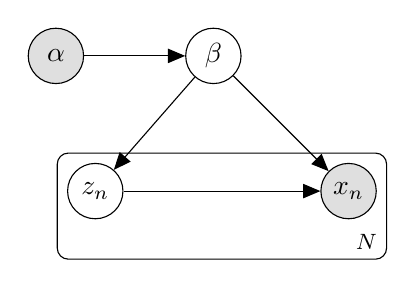
\begin{tikzpicture}
% Nodes
% parameters and data
\node[latent](z){$z_n$};
\node[obs, above = of z, xshift=-0.5cm](alpha)    {$\alpha$}; %
\node[latent, above = of z, xshift = 1.5cm](beta){$\beta$};
\node[obs, right = of z, xshift=1.5cm](x){$x_n$};

\edge{alpha}{beta};
\edge{beta}{z};
\edge{z}{x};
\edge{beta}{x};


\plate[]{plate}{
(z)(x)
}{$N$};


\end{tikzpicture}
\end{figure}
The joint distribution is 
$$p(x,z,\beta | \alpha)=p(\beta | \alpha)\prod_{n=1}^N p(x_n,z_n | \beta)$$
The task is to infer the posterior distribution of local latent variables $z$ and the global variable $\beta$ given the data $x$. 
$$p(z, \beta | x, \alpha)$$
\end{frame}

\begin{frame}{Two methods}
To do inference, there are usually two methods:
\begin{enumerate}
\item MCMC, the basic idea is to construct a Markov chain such that if we sample points on this chain. We will get the posterior distribution.
\item Variational Inference
\end{enumerate}


\end{frame}
\begin{frame}{Introduction}
Here is a PGM of LDA.

\begin{figure}[H]
    \centering
    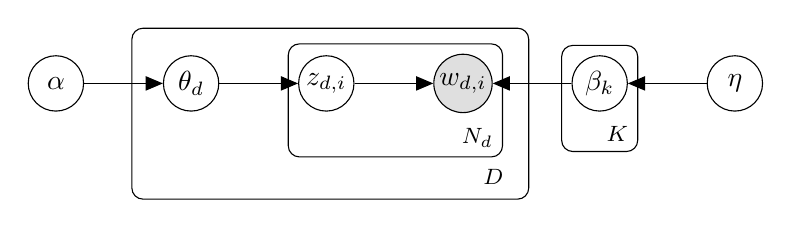
\begin{tikzpicture}
      % Nodes
      % parameters and data
      \node[latent]           (alpha)    {$\alpha$}; %
      \node[latent, right= of alpha]  (theta) {$\theta_d$};
      \node[latent, right= of theta]  (z) {$z_{d,i}$};
      \node[obs, right = of z]  (w) {$w_{d,i}$};
      \node[latent, right = of w]  (phi) {$\beta_k$};
      \node[latent, right = of phi]  (beta) {$\eta$};
      % edges
       \edge{alpha}{theta};
       \edge{theta}{z};
       \edge{z}{w};
       \edge{phi}{w};
       \edge{beta}{phi};
     % Plates
      {
       \tikzset{plate caption/.append style={below=20pt of #1.south east}}
       \plate[inner ysep=7pt, inner xsep=10pt, xshift=-1pt, yshift=2pt] {plate1} {(theta)(z)(w)} {$D$};
      }
    
      \plate[]{plate2}{
        (z)(w)
      }{$N_d$};
    
      \plate[]{plate3}{
        (phi)
      }{$K$};
    \end{tikzpicture}
    \end{figure}
We want to sample the posterior distribution of the latent variable $z_{d,i}$ given $w_{d,i}$. One method is gibbs sampling, in every iteration, we sample $z_i$ from distribution $p(z_i | z_{\neg i}, w)$.
The joint distribution is 
$$p(w,z | \alpha, \beta) = p(w | z, \beta) p(z | \alpha)$$
\end{frame}
\begin{frame}{Posterior predictive of Dirichlet-Multinomial}
Suppose we have dirichlet prior distribution,
$$p(\theta | \alpha) = \text{Dir}(\theta | \alpha) \propto \prod_{k=1}^K \theta_i^{\alpha_i - 1}$$

\end{frame}
\begin{frame}[allowframebreaks]{Joint distribution}
The joint distribution is $p(w,z | \alpha, \beta) = p(w | z, \beta) p(z | \alpha)$. The first part is

$$p(w | z, \beta) = \int_{\phi_{1 : K}} p(w | z, \phi_{1 : K})p(\phi_{1 : K} | \beta)d \phi_{1 :K}$$
Let's see $p(w | z, \phi_{1 : K})$ first, 
$$p(w | z, \phi_{1 : K}) = \prod_{i=1}^W \phi_{z_i, w_i}$$
Or we can rephrase it in another way, where we classify it by topic.
$$p(w | z, \phi_{1 : K}) = \prod_{i=1}^W \phi_{z_i, w_i} = \prod_{k=1}^K \prod_{v=1}^V \phi_{k,v}^{n_k^{(v)}}$$
And $$p(\phi_{1 : K} | \beta) = \prod_{k=1}^K \prod_{v=1}^V \phi_{k,v}^{\beta_v - 1} $$
Adding these two together, we have
$$p(w | z, \beta) = \prod_{k=1}^K \frac{B(n_k + \beta)}{B(\beta)}$$
$n_k$ represents the word apperance frequencies in topic $k$.
The topic distribution $p(z | \alpha)$ can be derived similarly,
$$p(z | \alpha) = \prod_{d=1}^D\frac{B(n_d + \alpha)}{B(\alpha)}$$
So the conditional distribution is
$$p(z,w | \alpha, \beta) = \prod_{k=1}^K \frac{B(n_k + \beta)}{B(\beta)}\prod_{d=1}^D\frac{B(n_d + \alpha)}{B(\alpha)}$$
$$p(z_i = k | z_{\neg i}, w, \alpha, \beta) = \frac{p(w,z) | \alpha, \beta}{p(w, z_{\neg i} | \alpha, \beta)} \propto p(w,z | \alpha, \beta) $$
Thus we just sample the $z_i$ according to the conditional distribution
$$p(z_i = k | z_{\neg i}, w, \alpha, \beta) \propto \prod_{k=1}^K \frac{B(n_k + \beta)}{B(\beta)}\prod_{d=1}^D\frac{B(n_d + \alpha)}{B(\alpha)}$$
We shall check out what is the same and what is different for different $k$ where $z_i = k$. As a result, it can be shown that 
$$p(z_i = k | z_{\neg i}, w, \alpha, \beta) \propto \Gamma(n_{k, w_i}^{\neg i}) \Gamma(n_{d, k}^{\neg i})$$
The symbol here is quite messy, if you have question, please feel free to contact me. $n_{k, w_i}^{\neg i}$ means except for this word, the frequency of word $w_i$ in topic $k$. And $n_{d, k}^{\neg i}$ means that except for this word, the frequency of word in document $d$ in topic $k$.
This is \text{collapsed Gibbs sampling}. In implementing this, \textbf{what we need to do is keeps sampling} $z$, and that is enough.
And after the sampling is done, the multinomial parameters can be derived as follows
$$p(\theta_d | w, z, \alpha) \sim \text{Dir}(\theta_m | n_m + \alpha)$$
$$p(\phi_d | w, z, \beta) \sim \text{Dir}(\phi_d | n_d + \beta) $$
\end{frame}


\begin{frame}[allowframebreaks]{Evidence Lower Bound(ELBO)}
    $$\ln (p(X)) = \ln (\frac{p(X,Z)}{q(Z)} - \ln (\frac{p(Z|X)}{q(Z)})$$
    Taking the expecttion w.r.t $q(Z)$ on both sides
    \begin{align*}
    \ln (P(X)) & = \int q(Z) \ln (\frac{p(X,Z)}{q(Z)} dZ - \int q(Z)\ln (\frac{p(Z|X)}{q(Z)}) dZ \\
    & = \mathcal{L}(q) + KL(q || p)
    \end{align*}
    Alternative derivation using Jensen's inequality:
    \begin{align*}
    \ln (X) & = \ln \int_Z p(X,Z) dZ \\
    & = \ln \int_Z p(X,Z) \frac{q(Z)}{q(Z)} dZ \\
    & = \ln \mathbb{E}_{Z \sim q(Z)} [\frac{p(X,Z)}{q(Z)}] \\
    & \ge \ln \mathbb{E}_{Z \sim q(Z)} [\frac{p(X,Z)}{q(Z)}] \\
    & = \int q(Z) \ln (\frac{p(X,Z)}{q(Z)}) dZ
    \end{align*}
    Which is $\mathcal{L}(q)$. We are interested in finding the lower bound of $\ln(X)$. And when the selected $q(Z)$ is closest to $p(Z|X)$, the KL divergence is 0, therefore, minimum is achieved.
    There are two typical approaches of get $q(Z)$,
    \begin{itemize}
    \item Assume that $q(Z)$ has some factorization $q(Z) = \prod_{i=1}^M q_i(Z_i)$.
    \item Assume $q(Z)$ is in some families of distribution(e.g. exponential families).
    \end{itemize}
    \end{frame}
    \begin{frame}{Factorization form}
    Assume that $q(z)$ can be factorized as follows, $q(z) = \sum_{i=1}^M q_i(z_i)$
    \begin{align*}
    \mathcal{L}(q) & = \int q(z) \ln p(x,z) dz - \int q(z) \ln q(z) dz \\
    & = \int \prod_{i=1}^M q_i(z_i) \ln p(x,z) dz - \int \prod_{i=1}^M q_i(z_i) \sum_{i=1}^M \ln q_i(z_i) dz \\
    \end{align*}
    If we just optimize $q_i(z_i)$ one at a time as follows,(Note that it is a iterative process)
    \begin{align*}
    \mathcal{L}(q) & = \int q_i(z_i)\mathbb{E}_{z_{\neg i}}[\ln p(x,z)]dz_i - \int q_i(z_i) \ln q_i(z_i) dz_i\\
    & = \int q_i(z_i)\ln \tilde{p}(x,z_i)dz_i - \int q_i(z_i) \ln q_i(z_i) dz_i \\
    & = \int q_i(z_i) \ln \frac{\tilde{p}(x,z_i)}{q_i(z_i)} = KL[\tilde{p}(x,z_i) || q_i(z_i)]
    \end{align*}
    \end{frame}
    
    \begin{frame}[allowframebreaks]{Exponential family distribution}
    Exponential family distribution is a rich family of distribution which computational tractable which is suitable for variational inference.
    $$p(x) = h(x) e^{\eta^\top T(x) - A(\eta)}$$
    Probability distribution in exponential family has several advantages. We can see that it is very easy to get the maximum likelihood estimation.
    
    $$\ln \prod_{i=1}^N p(x_i | \eta) = \sum_{i=1}^N \ln h(x_i) + \eta^\top (\sum_{i=1}^N T(x_i)) - N A(\eta)$$
    So if we want to get the maximum likelihood estimation,
    $$\frac{dA(\eta)}{d \eta} = \frac{\sum_{i=1}^N T(x_i)}{N}$$
    
    \framebreak
    
    Let's see an example of one-dimensional Gaussian distribution,
    $$\mathcal{N}(x | \mu, \sigma^2) = (2 \pi \sigma^2)^{-\frac{1}{2}} \exp(-\frac{(x - \mu)^2}{2 \sigma^2})$$
    We transform it into the exponential family distribution,
    $$p(x | \eta) = h(x) e^{\eta^\top T(x) - A(\eta)} = \exp(\mat{x \\ x^2}^\top \mat{\eta_1 \\ \eta_2} - (\frac{-\eta_1^2}{4\eta_2} + \frac{1}{2}\ln \eta_2) - \frac{1}{2} \ln 2\pi)$$
    $$\mat{\eta_1 \\ \eta_2} = \mat{\frac{\mu}{\sigma^2} \\ -\frac{1}{2\sigma^2}}$$
    and 
    $$A(\eta) = \frac{-\eta_1^2}{4\eta_2} + \frac{1}{2}\ln \eta_2 \qquad T(x) = \mat{x \\ x^2} \qquad \theta = \mat{\mu \\ \sigma^2} = \mat{\frac{-\eta_1}{2\eta_2} \\ \frac{-1}{2\eta_2}}$$
    
    \framebreak
    
    Now we use the previous conclusion to get the maximum likelihood estimation.
    
    $$\frac{dA(\eta)}{d \eta} = \frac{\sum_{i=1}^N T(x_i)}{N}$$
    $$A(\eta) = \frac{-\eta_1^2}{4\eta_2} + \frac{1}{2}\ln \eta_2$$
    $$\mat{-\frac{\eta_1}{2\eta_2} \\ \frac{\eta_1^2}{4\eta_2^2} + \frac{1}{2\eta_2}} = \mat{\frac{\sum_{i=1}^N x_i}{N} \\ \frac{\sum_{i=1}^N x_i^2}{N}}$$
    With 
    $$\theta = \mat{\mu \\ \sigma^2} = \mat{\frac{-\eta_1}{2\eta_2} \\ \frac{-1}{2\eta_2}}$$
    it is easy to solve $\mu$ and $\sigma^2$.
    Moreover, conjugate distribution in exponential familiy distribution are easy to compute.
    
    \framebreak
    
    We now show one important property of exponential family distribution that, for $$p(x | \lambda) = h(x) \exp (T(x)^\top \lambda - A_g(\lambda))$$ We have $$\nabla_\lambda A_g(\lambda) = \mathbb{E}_{p(x | \lambda)}[T(x)]$$
    From 
    $$\int_x p(x | \lambda) dx = \int_x h(x) \exp (T(x)^\top \lambda - A_g(\lambda))dx = 1$$
    \begin{gather*}
    \nabla_\lambda \int_x h(x) \exp (T(x)^\top \lambda - A_g(\lambda))dx = 0 \\
    \int_x \nabla_\lambda h(x) \exp (T(x)^\top \lambda - A_g(\lambda))dx = 0 \\
    \int_x \nabla_\lambda h(x) \exp (T(x)^\top \lambda - A_g(\lambda))dx = 0 \\
    \int_x p(x | \lambda)(T(x) - \nabla A_g(\lambda))dx = 0 \\
    \nabla_\lambda A_g(\lambda) = \mathbb{E}_{p(x | \lambda)}[T(x)]
    \end{gather*}
    Thus the equation holds.
    
    \end{frame} 
\begin{frame}[allowframebreaks]{Variational Inference}
    Now let's see how to implement do variational inference for the following model.
    \begin{figure}[H]
\centering
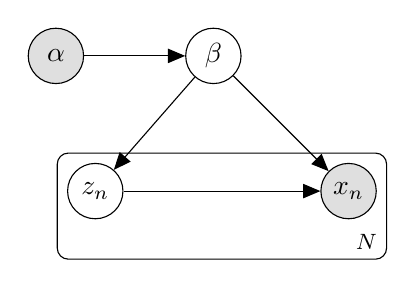
\begin{tikzpicture}
% Nodes
% parameters and data
\node[latent](z){$z_n$};
\node[obs, above = of z, xshift=-0.5cm](alpha)    {$\alpha$}; %
\node[latent, above = of z, xshift = 1.5cm](beta){$\beta$};
\node[obs, right = of z, xshift=1.5cm](x){$x_n$};

\edge{alpha}{beta};
\edge{beta}{z};
\edge{z}{x};
\edge{beta}{x};


\plate[]{plate}{
(z)(x)
}{$N$};


\end{tikzpicture}
\end{figure}
    The joint distribution is 
    $$p(x,z,\beta | \alpha)=p(\beta | \alpha)\prod_{n=1}^N p(x_n,z_n | \beta)$$
    We make the following assumptions, the conditional distribution belongs to exponential family distribution,
    $$p(\beta | x,z,\alpha)=h(\beta)\exp(\eta_g (x,z,\alpha)^\top T(\beta)-A_g(\eta_g(x,z,\alpha)))$$
    and
    $$\scriptstyle p(z_{nj}|x_n,z_{n,\neg j},\beta)=h(z_{nj})\exp(\eta_l(x_n,z_{n,\neg j},\beta)^\top T(z_{nj})-A_l(\eta_l(x_n,z_{n,\neg j},\beta)))$$
    The evidence lower bound is
    $$\mathcal{L}(q)=\mathbb{E}_q[\log p(x,z,\beta)]-\mathbb{E}_q[\log q(z,\beta)]$$
    We select the distribution $q$ such that it is both expressive and easier to optimize, (Note that we only restrict the function form for $p$, but have not specifies the factorization form of $p$.)
    $$q(z,\beta)=q(\beta|\lambda)\prod_{n=1}^N \prod_{j=1}^J q(z_{nj}|\phi_{nj})$$
    Other than the factorization of $q(z,\beta)$, we restrict $q(z, \beta)$ and $q(z_{nj} | \phi_{nj})$.
    $$q(\beta | \lambda)=h(\beta)\exp(\lambda^\top T(\beta)-A_g(\lambda))$$
    $$q(z_{nj}|\phi_{nj})=h(z_{nj})\exp(\phi_{nj}^\top T(z_{nj})-A_l(\phi_{nj}))$$
    Now let's alter the parameter $\lambda, \phi$ to maximize the ELBO.
    Rather than $\mathcal{L}(q)$, we can write it as $\mathcal{L}(\lambda, \phi)$.
    It turns out we can optimize $\lambda$ and $\phi$ in turn.  We first fix $\phi$ and optimize $\lambda$. 
    
    \begin{align*}
    \mathcal{L}(q)& =\mathbb{E}_q[\log p(x,z,\beta)]-\mathbb{E}_q[\log q(z,\beta)] \\
    & = \mathbb{E}_q[\log p(\beta | x,z)] + \underbrace{\mathbb{E}_q[\log p(x,z)]}_{\text{not related to }\beta}-\mathbb{E}_q[\log q(z,\beta)] \\
    & = \mathbb{E}_q[\log h(\beta)] + \mathbb{E}_q[\eta_g (x,z)]^\top \mathbb{E}_q[T(\beta)]-\mathbb{E}_q[A_g(\eta_g(x,z))]  \\ 
    & \quad  - \mathbb{E}_q[\log h(\beta)] - \mathbb{E}_q[T(\beta)^\top \lambda] +  \mathbb{E}[A_g(\lambda)] \\
    & = \mathbb{E}_q[\eta_g (x,z)]^\top\mathbb{E}_q[T(\beta)]-\mathbb{E}_q[A_g(\eta_g(x,z))] - \mathbb{E}_q[T(\beta)^\top \lambda] \\ 
    & \quad + \mathbb{E}[A_g(\lambda)] \\ 
    & = \mathbb{E}_q[\eta_g (x,z)]^\top\mathbb{E}_q[T(\beta)] - \mathbb{E}_q[T(\beta)]^\top\lambda + A_g(\lambda) \\
    & = \nabla_\lambda A_g(\lambda)^\top(\mathbb{E}_{q(z | \phi)}[\eta_g (x,z)] - \lambda) + A_g(\lambda)
    \end{align*}
    Maximize w.r.t $\mathcal{L}(\lambda)$ a.k.a $\mathcal{L}(q)$, $\frac{d\mathcal{L}(\lambda)}{d \lambda} = 0$, we have 
    $$\nabla^2_\lambda A_g(\lambda)^\top(\mathbb{E}_{q(z | \phi)}[\eta_g (x,z)] - \lambda) = 0$$
    
    \framebreak 
    Assume that $\nabla^2_\lambda A_g(\lambda) \neq 0$, so we have
    $$\mathbb{E}_{q(z | \phi)}[\eta_g (x,z)] - \lambda = 0$$
    That's cool! Right? What have we done so far?
    \begin{itemize}
    \item We first specifies a graphical model, and specifies the latent variables e.g. $z, \beta$.
    \item We define the distribution so that the conditional distribution for latent varaibels given other variables is always exponential family distribution.
    \item For joint distribution of latent variable e.g. $q(z, \beta)$, we assume that $q(z, \beta)$ factorizes into $q(z | \lambda)q(\beta | \phi)$. 
    \item Then, we have a very nice conclusion from our previous lengthy derivation that if we optimize the parameters e.g. $\lambda, \phi$ one by one, we just do it in this way. Repeat between $\lambda = \mathbb{E}_{q(z | \phi)}[\eta_g (x,z)]$ and $\phi = \mathbb{E}_{q(z | \lambda)}[\eta_l (x,\beta)]$ which is \textbf{set the parameter to be the expectation of natural prameter conditioning on all other latent variables}.
    \end{itemize}
    \end{frame}
    
    \begin{frame}[allowframebreaks]{Variational Inference for LDA}
    We will now do variational inference for the following model,
    
\begin{figure}[H]
    \centering
    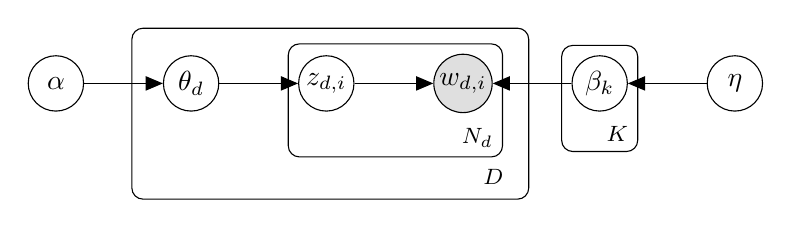
\begin{tikzpicture}
      % Nodes
      % parameters and data
      \node[latent]           (alpha)    {$\alpha$}; %
      \node[latent, right= of alpha]  (theta) {$\theta_d$};
      \node[latent, right= of theta]  (z) {$z_{d,i}$};
      \node[obs, right = of z]  (w) {$w_{d,i}$};
      \node[latent, right = of w]  (phi) {$\beta_k$};
      \node[latent, right = of phi]  (beta) {$\eta$};
      % edges
       \edge{alpha}{theta};
       \edge{theta}{z};
       \edge{z}{w};
       \edge{phi}{w};
       \edge{beta}{phi};
     % Plates
      {
       \tikzset{plate caption/.append style={below=20pt of #1.south east}}
       \plate[inner ysep=7pt, inner xsep=10pt, xshift=-1pt, yshift=2pt] {plate1} {(theta)(z)(w)} {$D$};
      }
    
      \plate[]{plate2}{
        (z)(w)
      }{$N_d$};
    
      \plate[]{plate3}{
        (phi)
      }{$K$};
    \end{tikzpicture}
    \end{figure}
    Here is a pipeline for doing variational inference.
    \begin{itemize}
    \item The graphical model encodes the conditional independence information of the model.
    \item We assign the exponential family distribution to the distribution such that we can get exponential family conditional distribution for future ease.
    \item Write the $q$ distribution for each full conditional distribution and do optimization.
    \end{itemize}
    
    \framebreak
    For LDA,
    The document-topic distribution is 
    $$\theta_d \sim \text{Dir}(\alpha)$$
    The topic-word distribution is
    $$\phi_k \sim \text{Dir}(\beta)$$
    The topic assignment of each word is
    $$ z_{d,i} \sim \text{Mult}(\theta_d)$$
    And for each word, 
    $$ w_{d,i} \sim \text{Mult}(\theta_{z_{d,i}})$$
    
    \framebreak
    We have three kinds of latent variables, $\theta_d$, $z_{d,i}$ and $\phi_k$ respectively. We now derive the conditional distribution of these given all other variables.
    First, we derive the conditional distribution of $z_{d,n}$, it can be shown that the conditional distribution of $z_{d,n}$ is
    \begin{align*}
    & p(z_{d,n} = k | \theta_d, w_{d,n}, \phi_k)\\
    \propto \quad & p(w_{d,n} | z_{d,n} = k, \phi_k) p(z_{d,n} = k | \theta_d)\\
    = \quad & \phi_{k, w_{d,n}} \theta_{d,k} \\
    = \quad & \exp (\ln [\phi_{k, w_{d,n}}\theta_{d,k}])
    \end{align*}
    \framebreak
    
    For conditional distribution for the topic distribution of each document $\theta_d$, it can be shown that $$p(\theta_d | \text{all other variables}) = p(\theta_d | z_d)$$
    \begin{align*}
    & p(\theta_d | z_d) \\
    \propto \quad &  p(\theta_d | \alpha) \prod_{n=1}^{N_d} p(z_{d,n} | \theta_d)\\
    = \quad & \prod_{k=1}^K (\theta_{d,k}^{\alpha_k - 1} \prod_{n=1}^{N_d} \theta_{d,k}^{\delta(z_{d,n}, k)})\\
    = \quad & \prod_{k=1}^K (\theta_{d,k}^{\alpha_k - 1 + n_k}) \qquad \text{where } n_k = \sum_{n=1}^{N_d} \delta(z_{d,n}, k) \\
    = \quad & \exp (\sum_{k=1}^K (\alpha_k - 1 + n_k) \log \theta_{d,k}) 
    \end{align*}
    
    \framebreak
    
    For conditional distribution for the word distribution of each topic $\phi_k$,
    \begin{align*}
    & p(\phi_k | Z, W) \\
    \propto \quad &  p(\phi_{k,v} | \beta) \prod_{d=1}^D\prod_{n=1}^{N_d} p(w_{d,n} | \phi_k)^{\delta(z_{d,n}, k)}\\
    = \quad & \prod_{v=1}^V \phi_{k,v}^{\beta_v - 1}\prod_{d=1}^D\prod_{n=1}^{N_d} p(w_{d,n} | \phi_k)^{\delta(z_{d,n}, k)} \\
    = \quad & \prod_{v=1}^V \phi_{k,v}^{\beta_v - 1}\prod_{d=1}^D\prod_{n=1}^{N_d} \phi_{k, w_{d,n}}^{\delta(z_{d,n}, k)} \\
    = \quad & \exp (\sum_{v=1}^V (\beta_v - 1 +  n_v) \log \phi_{k,v}) 
    \end{align*}
    where $n_v$ is the number of occurence of word $v$ which belongs to topic $k$.
    
    So now we have the three conditional distribution of latent parameters. Now we can perform variational inference for our graphical model.
    
    \begin{gather*}
    p(z_{d,n} = k | \theta_d, w_{d,n}, \phi_k)  =  \exp (\ln [\beta_{k, w_{d,n}}\theta_{d,k}])\\
    p(\theta_d | z_d)  = \exp (\sum_{k=1}^K (\alpha_k - 1 + n_k) \log \theta_{d,k}) \\
    p(\beta_k | Z, W)  = \exp (\sum_{v=1}^V (\eta_v - 1 +  n_v) \log \beta_{k,v}) 
    \end{gather*}
    We assume that the variational function is in the form of 
    \begin{gather*}
    q(z_{d,n})=\text{Mult}(\phi_{d,n})\\
    q(\theta_d)=\text{Dir}(\gamma_d)\\
    q(\beta_k) = \text{Dir}(\lambda_k)
    \end{gather*}
    According to the property of exponential family, we have the following conclusion
    \begin{gather*}
    \eta(\phi_{d,n}) = \mathbb{E}_{q(\theta_d) q(\beta_k))}(\ln [\beta_{k, w_{d,n}\theta_{d,k}}])\\
    \eta(\gamma_d) = \mathbb{E}_{q(z_{d,n}) q(\beta_k))}(\mat{\alpha_1 - 1 + n_1 \cdots \alpha_K - 1 + n_K}^\top)\\
    \eta(\beta_k) = \mathbb{E}_{q(z_{d,n}) q(\theta_d))}(\mat{\eta_1 - 1 + n_1 \cdots \eta_V - 1 + n_V}^\top)
    \end{gather*}
    
    \framebreak
    \begin{align*}
    \eta(\phi_{d,n}) & = \mathbb{E}_{q(\theta_d) q(\beta_k))}(\ln [\beta_{k, w_{d,n}\theta_{d,k}}]) \\
    & = \mathbb{E}_{q(\theta_d)}[\ln \theta_{d,k}] + \mathbb{E}_{q(\beta_k)}[\ln \beta_{k, w_{d,n}}] \\ 
    & = \Psi(\gamma_{d,k}) - \Psi(\sum_{k=1}^K \gamma_{d,k}) + \Psi(\lambda_{k,w_{d,n}}) - \Psi(\sum_{v=1}^V \lambda_{k,v})
    \end{align*}
    $$\eta(\gamma_d) = \mat{\alpha_1 - 1 + \phi_{d,n}^1 \cdots \alpha_K 1 + \phi_{d,n}^K}^\top$$
    $$\eta(\beta_k) = \eta -1 + \sum_{d=1}^D\sum_{n=1}^N w_{d,n} \phi_{d,n}^k$$
    Huh! That's our updating rules for the variational inference for LDA.
    
    \end{frame}

\begin{frame}{Perplexity}
\end{frame}


\end{document}